%----------------------------------------------------------------
\subsection{Hardware}
\begin{wrapfigure}{r}{0.5\textwidth}
	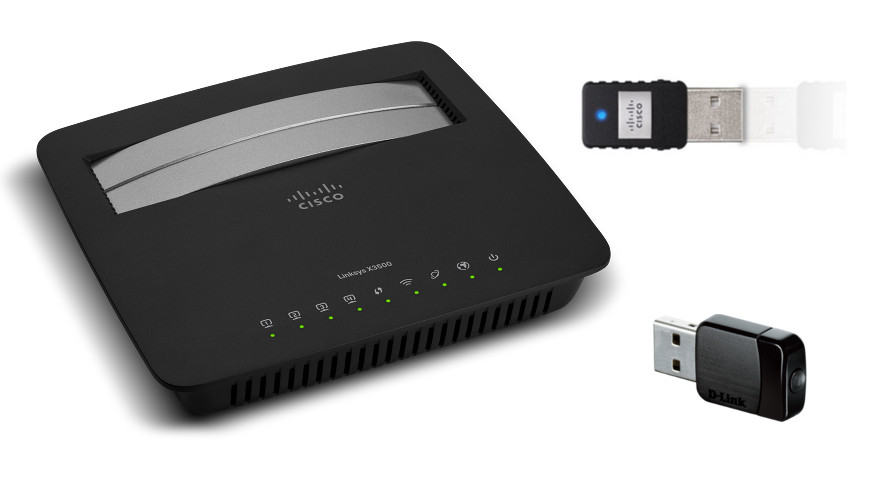
\includegraphics[width=0.5\textwidth]{../Images/c1/hardware_comm.jpg}
	\caption{WiFi PA and USB adapters}
	\label{fig:hardwareComm}
\end{wrapfigure}

This section briefly describes the architecture of communication. In order to be versatile and flexible, the experiments will use one router and one WiFi adapter per quadrotor. The flexibility became because with those devices is don't restrict the software, i. e., the whole system can be uses with GSM modules and cloud computation or inside a computer with simulated targets and persecutors (Quadrotors).


%% 666 TODO: cambiar imagen a la que debe ser!!!

%----------------------------------------------------------------
\subsection{Software, protocol and messages}

\begin{wrapfigure}{r}{0.5\textwidth}
	\begin{center}
		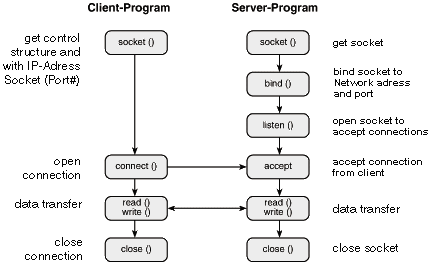
\includegraphics[width=0.5\textwidth, natwidth=448, natheight=263]{../Images/c1/socketstcpip.png}
	\end{center}
	\caption{Sockets and TCP-IP}
	\label{fig:socketstcpip}
\end{wrapfigure}

To communicate between devices every application (or program) use a sockets \cite{SocketWiki}. Particularly, an implementation developed initially for this project that can be found in BOViL \cite{BOViL}. Sockets are configured with the TCP/IP protocol \cite{TCPIP}. \\
Every step of the program, after the segmentation of the image, an array of centroids is generated that correspond to the targets detected by quadrotor's camera. This array is send throught the socket byte per byte (or character per character) following the format of the image \ref{fig:message_structure}. For example $\{14;01;123-231,142-22,...,600-232\}$

